\subsection*{Problema 08}
\textbf{Enunciado:} Calcular la integral:
\begin{align*}
\int \dfrac{dx}{\cos x + \cot x}
\end{align*}

\textbf{Solución:} 
Siguiendo las indicaciones, expresamos la cotangente en términos de seno y coseno:
\begin{align*}
\cot x = \dfrac{\cos x}{\sin x}
\end{align*}

Sustituimos esta identidad en el denominador de la integral original:
\begin{align*}
\int \dfrac{dx}{\cos x + \dfrac{\cos x}{\sin x}}
\end{align*}

Sacamos factor común $\cos x$ en el denominador:
\begin{align*}
\int \dfrac{dx}{\cos x \left(1 + \dfrac{1}{\sin x}\right)}
\end{align*}

Encontramos denominador común dentro del paréntesis:
\begin{align*}
\int \dfrac{dx}{\cos x \left(\dfrac{\sin x + 1}{\sin x}\right)}
\end{align*}

Aplicamos la regla de la división de fracciones para llevar $\sin x$ al numerador:
\begin{align*}
\int \dfrac{\sin x \, dx}{\cos x (1 + \sin x)}
\end{align*}

Ahora, aplicamos la sustitución sugerida:
\begin{align*}
u = \sin x, \quad du = \cos x \, dx
\end{align*}

Recordamos la identidad trigonométrica fundamental para expresar el coseno cuadrado en términos del seno:
\begin{align*}
\cos^2 x = 1 - \sin^2 x = 1 - u^2
\end{align*}

Reescribimos la integral multiplicando numerador y denominador por $\cos x$:
\begin{align*}
\int \dfrac{\sin x \cos x \, dx}{\cos^2 x (1 + \sin x)}
\end{align*}

Sustituimos $u$, $du$ y $\cos^2 x$:
\begin{align*}
\int \dfrac{u \, du}{(1 - u^2)(1 + u)}
\end{align*}

Factorizamos la diferencia de cuadrados en el denominador:
\begin{align*}
\int \dfrac{u \, du}{(1 - u)(1 + u)^2}
\end{align*}

Descomponemos en fracciones parciales:
\begin{align*}
\dfrac{u}{(1-u)(1+u)^2} = \dfrac{A}{1-u} + \dfrac{B}{1+u} + \dfrac{C}{(1+u)^2}
\end{align*}

Resolviendo para los coeficientes, obtenemos:
\begin{align*}
A = \dfrac{1}{4}, \quad B = -\dfrac{1}{4}, \quad C = -\dfrac{1}{2}
\end{align*}

Sustituimos los coeficientes e integramos cada término por separado:
\begin{align*}
\int \left( \dfrac{1/4}{1-u} - \dfrac{1/4}{1+u} - \dfrac{1/2}{(1+u)^2} \right) du
\end{align*}

Integrando paso a paso:
\begin{align*}
= -\dfrac{1}{4}\ln|1-u| - \dfrac{1}{4}\ln|1+u| + \dfrac{1}{2(1+u)} + C
\end{align*}

Agrupamos los logaritmos utilizando las propiedades de los mismos:
\begin{align*}
= -\dfrac{1}{4}\ln|1-u^2| + \dfrac{1}{2(1+u)} + C
\end{align*}

Regresamos a la variable original $u = \sin x$:
\begin{align*}
= -\dfrac{1}{4}\ln|1-\sin^2 x| + \dfrac{1}{2(1+\sin x)} + C
\end{align*}

Dado que $1-\sin^2 x = \cos^2 x$, la solución final es:
\begin{align*}
= -\dfrac{1}{2}\ln|\cos x| + \dfrac{1}{2(1+\sin x)} + C
\end{align*}

\begin{figure}[H]
	\centering
	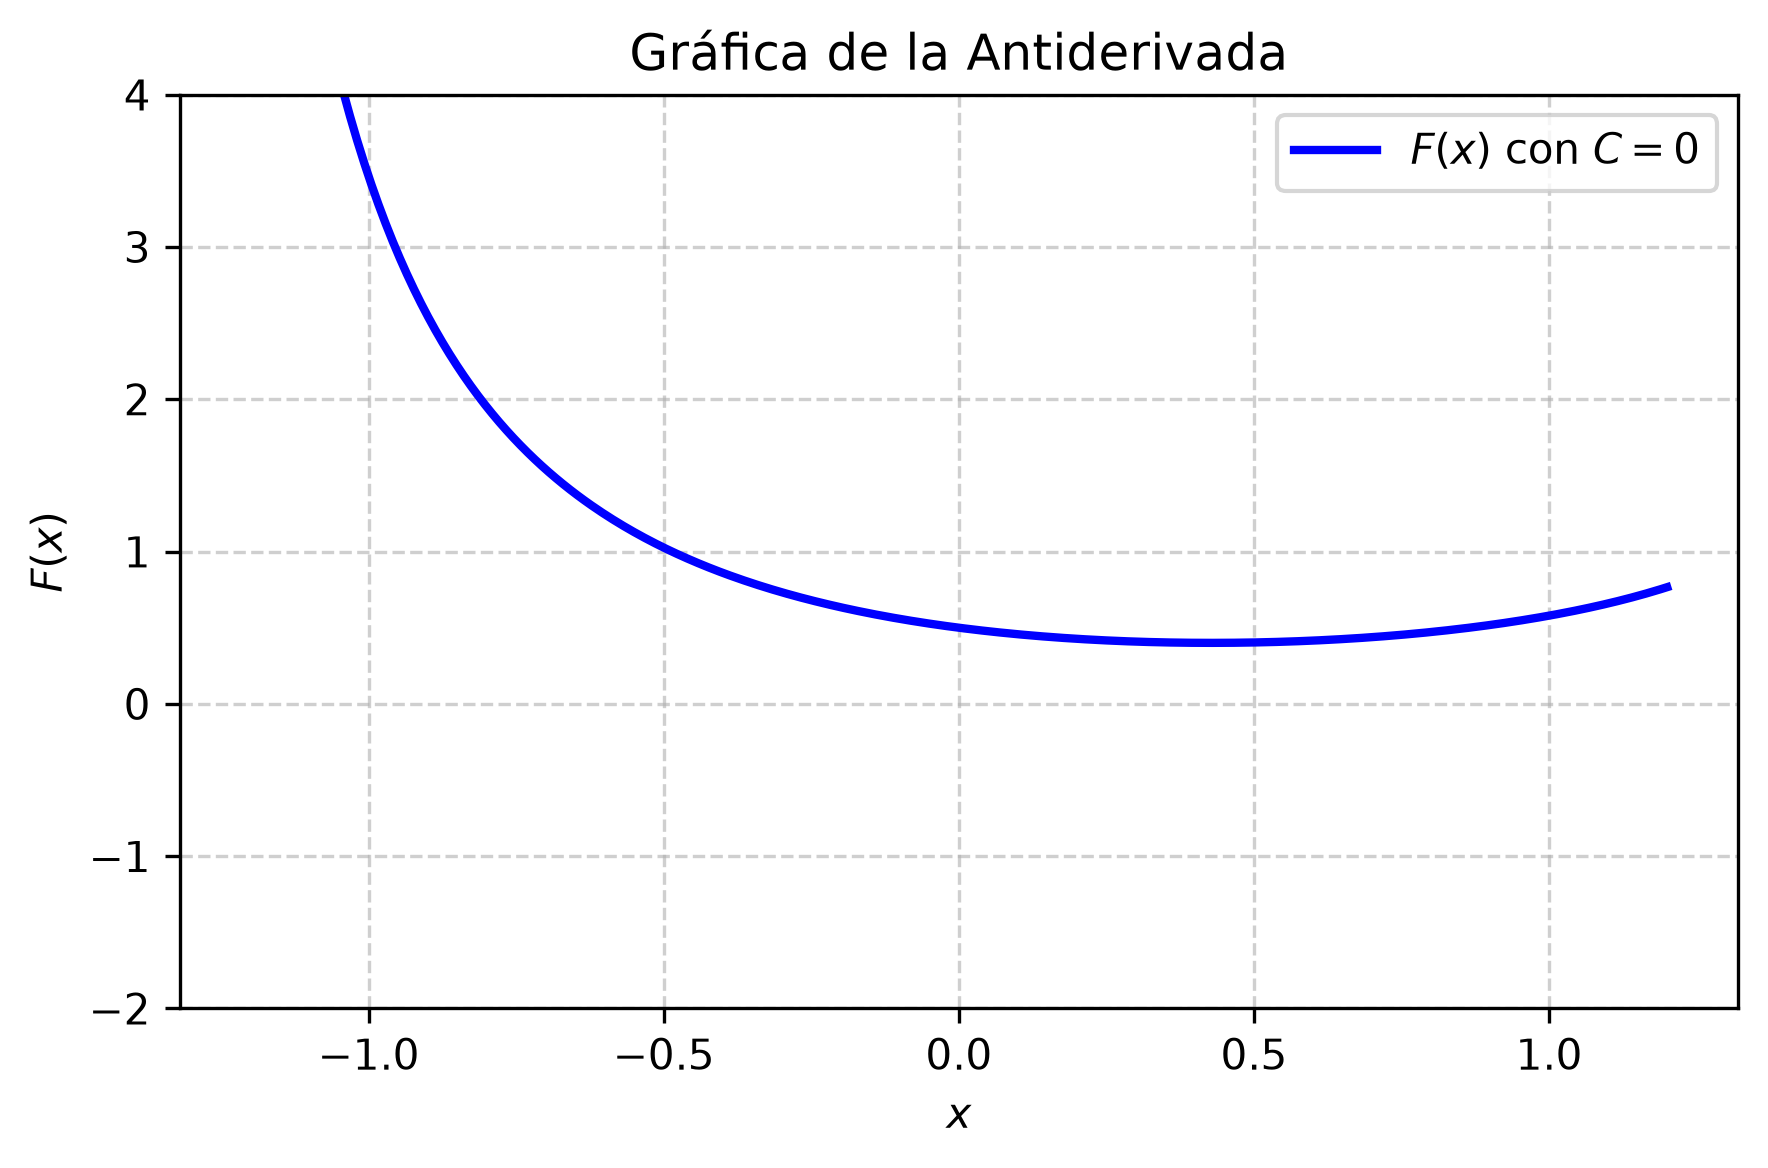
\includegraphics[width=\columnwidth]{semana_04/graficas/SEM04_P08_grafica.png}
	\caption{Representación gráfica de $f(x)$ y su antiderivada $F(x)$ evaluada para la constante de integración $C = 0$ (Problema 08).}
	\label{fig:problema08}
\end{figure}
